\documentclass[arhiv]{../izpit}
\usepackage{fouriernc}
\usepackage{tikz}

\begin{document}

\izpit{Programiranje I: 1.\ izpit}{2.\ februar 2016}{
  Čas reševanja je 150 minut.
  Doseženih 80 točk šteje za maksimalno oceno.
  \textbf{Funkcij v Haskellu ne pozabite opremiti z ustrezno signaturo.}
  Veliko uspeha!
}

%%%%%%%%%%%%%%%%%%%%%%%%%%%%%%%%%%%%%%%%%%%%%%%%%%%%%%%%%%%%%%%%%%%%%%
\naloga[Funkcije, 30 točk]

\podnaloga[10 točk]
V Haskellu sestavite funkcijo \verb|naloga1a|, ki na danem elementu zaporedoma uporabi vse funkcije iz danega seznama.
Na primer:
\begin{verbatim}
naloga1a [negate, (+ 1), subtract 3, (2 -), (* 2)] 5
\end{verbatim}
vrne $18$, saj je $(2 - (((-5) + 1) - 3)) \cdot 2 = 18$.

\podnaloga[10 točk]
Sestavite funkcijo \verb|naloga1b|, ki deluje podobno kot prejšnja, le da funkcijo uporabi na elementu le tedaj, kadar bi se s tem povečala vrednost.
Na primer:
\begin{verbatim}
naloga1b [negate, (+ 1), subtract 3, (2 -), (* 2)] 5
\end{verbatim}
vrne $12$, saj vrednost povečata le funkciji \verb|(+ 1)| in \verb|(* 2)|.
Pozor, pri različnih elementih vrednost povečajo različne funkcije.
Na primer:
\begin{verbatim}
naloga1b [negate, (+ 1), subtract 3, (2 -), (* 2)] (-3)
\end{verbatim}
vrne $8$, saj vrednost tokrat povečajo funkcije \verb|negate|, \verb|(+ 1)| in \verb|(* 2)|.

\podnaloga[10 točk]
Sestavite še funkcijo \verb|naloga1c|, ki deluje podobno kot prejšnji, le da uporabi tiste funkcije, s katerimi doseže največji možen rezultat.
Na primer:
\begin{verbatim}
naloga1c [negate, (+ 1), subtract 3, (2 -), (* 2)] 5
\end{verbatim}
vrne $20$, saj največji možen rezultat dosežemo kot $(2 - ((-5) - 3)) \cdot 2 = 20$.


%%%%%%%%%%%%%%%%%%%%%%%%%%%%%%%%%%%%%%%%%%%%%%%%%%%%%%%%%%%%%%%%%%%%%%
\naloga[Drobencljava podzaporedja, 20 + 10 točk]

Pravimo, da je zaporedje \emph{drobencljavo}, če se vsaka dva zaporedna člena med seboj po absolutni vrednosti razlikujeta za natanko $1$. Na primer, zaporedje $1, 2, 3, 2$ je drobencljavo, zaporedje $1, 2, 3, 1$ pa ne, ker se tretji in četrti člen razlikujeta za $2$.

\podnaloga[10 točk]
  Sestavite funkcijo \texttt{naloga2a}, ki učinkovito izračuna število vseh nepraznih drobencljavih podzaporedij danega zaporedja.
  Na primer, v zaporedju $1, 2, 3, 1$ je $9$ takih podzaporedij:
  \[
    1; \quad 2; \quad 3; \quad 1; \quad 1, 2; \quad 2, 3; \quad 2, 1; \quad 1, 2, 1; \quad 1, 2, 3.
  \]
  Bodite pozorni na to, da se lahko kakšno podzaporedje v danem zaporedju pojavi tudi večkrat, ter na to, da niso vsa podzaporedja nujno strnjena. V komentarju kode tudi utemeljite, kakšna je časovna zahtevnost vaše rešitve.

\podnaloga[10 točk]
  Sestavite funkcijo \texttt{naloga2b}, ki učinkovito izračuna množico vseh \emph{različnih} drobencljavih podzaporedij danega zaporedja. V komentarju kode tudi utemeljite, kakšna je časovna zahtevnost vaše rešitve.

\podnaloga[+10 točk]
  Sestavite funkcijo \texttt{naloga2c}, ki izračuna dolžino najdaljšega \emph{strnjenega} drobencljavega podzaporedja, ki se začne in konča z istim številom. Vaša rešitev naj deluje v času $O(n)$, kjer je $n$ dolžina zaporedja.


%%%%%%%%%%%%%%%%%%%%%%%%%%%%%%%%%%%%%%%%%%%%%%%%%%%%%%%%%%%%%%%%%%%%%%
\naloga[Drevesa, 30 + 10 točk]

Neprazna dvojiška drevesa, v katerih so vrednosti spravljene zgolj v listih, lahko v Haskellu predstavimo s podatkovnim tipom:
\begin{verbatim}
data Drevo a = List a
             | Razvejano (Drevo a) (Drevo a)
\end{verbatim}
Na primer, drevo
\[
  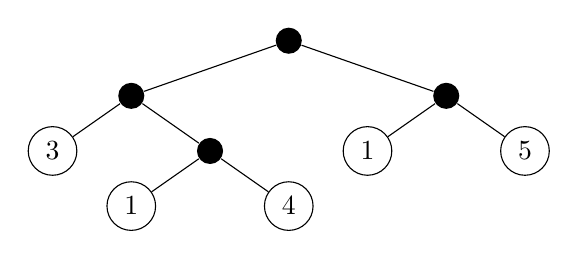
\begin{tikzpicture}[level distance=0.7cm,
    level 1/.style={sibling distance=4cm},
    level 2/.style={sibling distance=2cm},
    level 3/.style={sibling distance=2cm}
    ]
    \node[circle, fill] (d) {}
      child {node[circle, fill] {}
        child {node[circle, draw] {3}}
        child {node[circle, fill] {}
          child {node[circle, draw] {1}}
          child {node[circle, draw] {4}}
        }
      }
      child {node[circle, fill] {}
        child {node[circle, draw] {1}}
        child {node[circle, draw] {5}}
      };
  \end{tikzpicture}
\]
bi predstavili kot
\begin{verbatim}
Razvejano
  (Razvejano (List 3) (Razvejano (List 1) (List 4)))
  (Razvejano (List 1) (List 5))
\end{verbatim}

\podnaloga[10 točk]
  Sestavite funkcijo \verb|naloga3a|, ki vrne seznam vseh vrednosti, ki se pojavljajo v listih drevesa. Vrednosti naj bodo naštete od leve proti desni, kakor si sledijo v drevesu.
  Na primer, za zgornje drevo bi funkcija vrnila seznam $[3,1,4,1,5]$.

\podnaloga[10 + 10 točk]
  Sestavite funkcijo \verb|naloga3b|, ki vrne drevo z enako obliko kot dano drevo, le da so vse vrednosti v listih zamenjane z največjo vrednostjo. Na primer, za zgornje drevo bi funkcija vrnila drevo:
  \[
    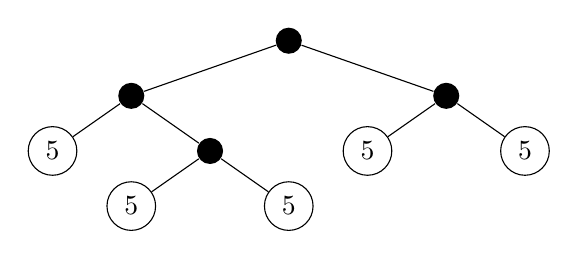
\begin{tikzpicture}[level distance=0.7cm,
      level 1/.style={sibling distance=4cm},
      level 2/.style={sibling distance=2cm},
      level 3/.style={sibling distance=2cm}
      ]
      \node[circle, fill] (d) {}
        child {node[circle, fill] {}
          child {node[circle, draw] {5}}
          child {node[circle, fill] {}
            child {node[circle, draw] {5}}
            child {node[circle, draw] {5}}
          }
        }
        child {node[circle, fill] {}
          child {node[circle, draw] {5}}
          child {node[circle, draw] {5}}
        };
    \end{tikzpicture}
  \]
  Za dodatnih $10$ točk funkcijo napišite tako, da naredi \emph{zgolj en} obhod po drevesu.

\podnaloga[10 točk]
  Sestavite funkcijo \verb|naloga3c|, ki vrne drevo z enako obliko kot dano drevo, le da so vrednosti v listih zaporedoma zamenjane s tistimi v danem seznamu. Na primer, za zgornje drevo in seznam $[2,7,1,8,2]$ bi funkcija vrnila drevo:
  \[
  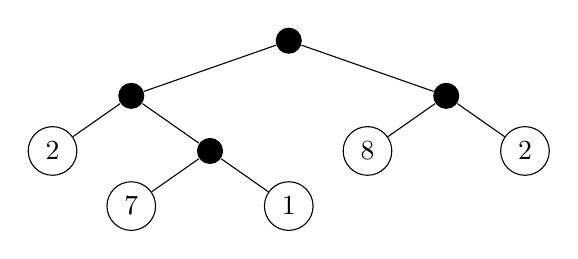
\begin{tikzpicture}[level distance=0.7cm,
    level 1/.style={sibling distance=4cm},
    level 2/.style={sibling distance=2cm},
    level 3/.style={sibling distance=2cm}
    ]
    \node[circle, fill] (d) {}
      child {node[circle, fill] {}
        child {node[circle, draw] {2}}
        child {node[circle, fill] {}
          child {node[circle, draw] {7}}
          child {node[circle, draw] {1}}
        }
      }
      child {node[circle, fill] {}
        child {node[circle, draw] {8}}
        child {node[circle, draw] {2}}
      };
  \end{tikzpicture}
\]
Če se število listov v drevesu ne ujema z dolžino seznama, naj funkcija javi napako.

  \noindent
  \textbf{Namig:} \verb|Drevo a -> [b] -> (Drevo b, [b])|


\end{document}